\documentclass{standalone}
\usepackage{tikz}
\usepackage{amsmath}
\usetikzlibrary{patterns,decorations.markings,backgrounds}
\usetikzlibrary{arrows.meta}
\usepackage{bm}

\def\a{-20}
\def\d{4}
\def\w{15}
\def\b{55}
\def\scale{0.2}
\def\eps{0.5}
\def\wall{0.5}
\def\h{20}

\def\aa{\a*\scale}
\def\dd{\d*\scale}
\def\ww{\w*\scale}
\def\bb{\b*\scale}
\def\hh{\h*\scale}

\def\textscale{2}

\begin{document}
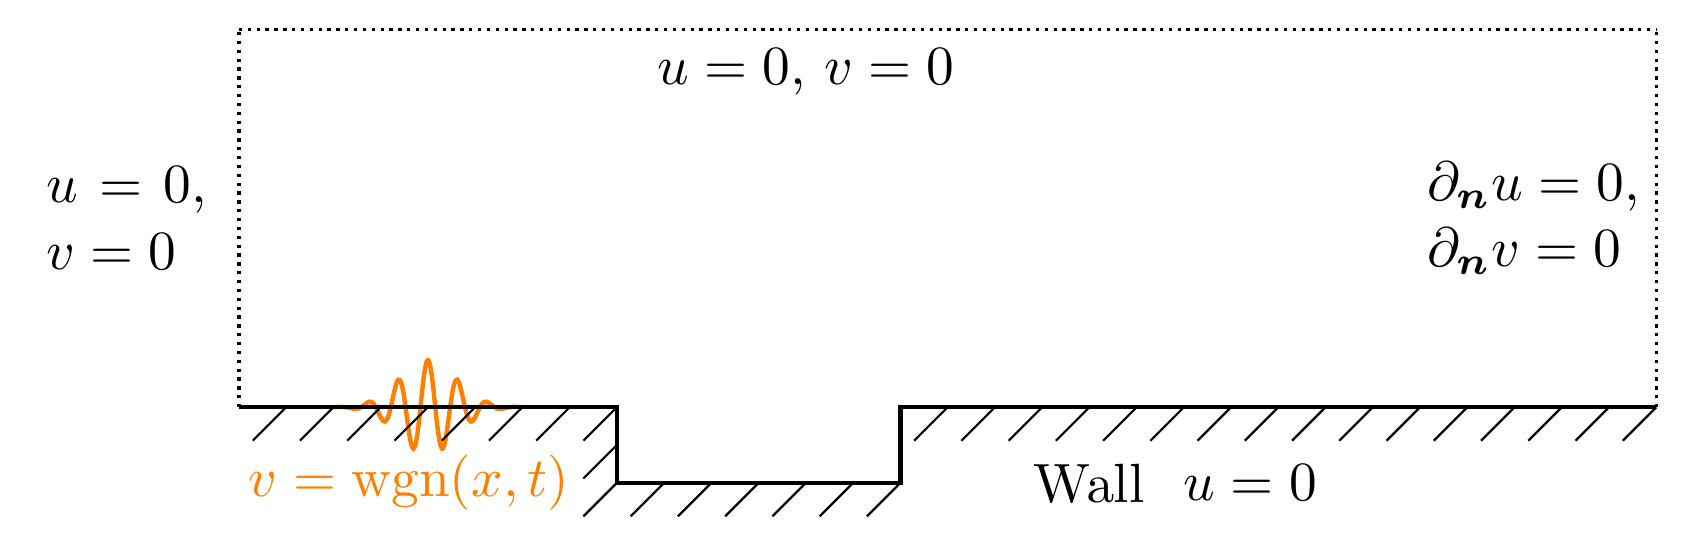
\begin{tikzpicture}[scale=1.2]

\draw[domain=-3:-1, samples=100, smooth,variable=\x, orange, ultra thick] plot ({\x}, {0.5*exp(-(\x+2)^2*5)*cos((\x+2)*180/3.14159)*cos(20*(\x+2)*180/3.14159)});

% Wall
\draw[ultra thick] (\aa,0) -- (0,0) -- (0,-\dd) -- (\ww,-\dd) -- (\ww,0) -- (\bb,0);

\def\lengthWall{0.5}
\foreach \x in {-3.5,-3,...,0,3.5,4,...,11} {
    \draw[thick] (\x,0) -- ++(225:\lengthWall); % Wall hatching
}
\foreach \x in {0,0.5,...,3} {
    \draw[thick] (\x,-\dd) -- ++(225:\lengthWall); % Wall hatching
}
\draw[thick] (0,-\dd/2) -- ++(225:\lengthWall); % Wall hatching

% BL Profile (velocity profile)
\def\BLxshift{-2cm}
% \draw [black, very thick, xshift=\BLxshift] plot [smooth, tension=0.5] coordinates { (-2,0) (-1.8,0.075) (-1.6,0.15) (-1.4, 0.225) (-1.2, 0.3) (-1.07,0.37) (-1,0.5) (-1, 1) (-1,1.25) (-1,1.5)};
% \draw [black, very thick, xshift=\BLxshift] (-2,0) -- (-2,1.5); % Left vertical line of BL profile
% \draw [-Latex, very thick, xshift=\BLxshift] (-2,1.5) -- (-1,1.5); % Arrow at the top of BL profile
% \draw [-Latex, very thick, xshift=\BLxshift] (-2,1.1125) -- (-1,1.125); % Arrow at the middle of BL profile
% \draw [-Latex, very thick, xshift=\BLxshift] (-2,0.75) -- (-1,0.75); % Arrow at the bottom of BL profile
% \draw [-Latex, very thick, xshift=\BLxshift] (-2,0.375) -- (-1.09,0.375); % Arrow at the bottom of BL profile
% Upper region
\draw[dotted,very thick] (\aa,\hh) -- (\bb,\hh); % Top boundary line
\draw[dotted,very thick] (\aa,0) -- (\aa,\hh); % Left boundary line
\draw[dotted,very thick] (\bb,0) -- (\bb,\hh); % Right boundary line

% Labels
\node[scale=\textscale] (W) at (5,-0.8) {Wall};
\node[xshift=\BLxshift,anchor=east,scale=\textscale,text width=1.3cm] at (-2,2) {$u=0$, $v=0$};
\node[scale=\textscale,anchor=west] at (W.east) {$u=0$};
\node[scale=\textscale, color=orange] at (-2.2,-0.8) {$v=\text{wgn}(x,t)$};
\node[scale=\textscale,anchor=north] at (2,\hh) {$u=0$, $v=0$};
\node[scale=\textscale,text width=1.35cm] at (9.7,2) {$\partial_{\bm{n}}u=0$, $\partial_{\bm{n}}v=0$};

\end{tikzpicture}
% \begin{tikzpicture}[scale=1]
%     % fill the rectangle
%   \draw[draw=black, line width = 1.25pt] (\aa, 0) -- (0,0) -- (0, -\dd) -- (\ww, -\dd) -- (\ww, 0) -- (\bb, 0);
%   \draw[pattern=north east lines] (\aa,0) rectangle (0,-\wall);  
%     % arrows
%   % \draw[stealth-stealth, thick] (\aa-\eps, 0) -- (\aa-\eps, \hh) node[midway, left] {$h$};
%   % \draw[stealth-stealth, thick] (\aa, -\eps) -- (0, -\eps) node[midway, below] {$L_i$};
%   % \draw[stealth-stealth, thick] (\ww, -\eps) -- (\bb, -\eps) node[midway, below] {$L_o$};
%   % \draw[stealth-stealth, thick] (0, -2*\eps) -- (\ww, -2*\eps) node[midway, below] {$w$};

%   % %depth
%   % \def\xloc{2*\ww}
%   % \def\len{0.5}
%   % % node ate the end
%   % \draw[-stealth, thick] (\xloc, -\len-\dd) -- (\xloc, -\dd) node[above, anchor=west] {$d$};
%   % \draw[stealth-, thick] (\xloc, 0) -- (\xloc, \len);
% \end{tikzpicture}
\end{document}
